\chapter{Fundamentação Teórica}\label{chapter:fundamentacao}
Neste capítulo pretende-se oferecer ao leitor uma visão geral das principais áreas nas quais esse trabalho está fundamentado. Mais especificamente, uma explanação sobre o~\ac{dp} seus sinais motores e os estágios da doença; uso da cinemetria como ferramenta para medição dos parâmetros cinemáticos do movimento humano; e os classificadores de dados para a identificação dos padrões presentes num conjunto de dados.


%A classificação mais ampla dos tipos de jogos separa-os em jogos para entretenimento, jogos sérios (serious games) e simuladores. Em (Narayanasamy, 2006) é dado o foco da diferença entre estes três tipos de jogos na forma como são desenvolvidos, ou seja, a diferença esta no foco de seu desenvolvimento, onde jogos de entretenimento seriam jogos desenvolvidos para a diversão do usuário, jogos sérios para aprendizagem de algo especifico e simuladores para o treinamento. Porém em (Johnston e Whitehead, 2009) é apresentada uma proposta um pouco diferente e mais interessante entre estas classificações. É proposto que estes jogos não se diferenciam em sua produção, mas sim pelos jogadores que o jogam. Uma forma de vermos  isto é pensarmos em um simulador de vôo. Se colocarmos uma criança nele, esta irá se divertir e considerar aquilo como um jogo de entretenimento, enquanto um piloto profissional o consideraria um simulador.
%RETIRADO DE - ATHUS



%Para esse trabalho, é considerada a definição estabelecida por Saywer (2004) e Prensky (2001) que definem os serious games como sendo aqueles que não têm como objetivo maior a diversão ou o entretenimento, e sim, o fim educacional ou a aprendizagem sobre determinado fato, informação ou habilidade. A diversão, neste caso, continua existindo como um fator essencial para engajar o jogador no ambiente de aprendizado.
%2.1.1 Classificação dos Serious Games Michael e Chen (2006) afirmam que os serious games se diferenciam dos jogos de entretenimento pelo seu propósito final, dessa forma, eles não representam um gênero específico. Tais jogos podem assumir qualquer gênero já definido da categoria de entretenimento, desde jogos de ação, aventura, corrida, estratégia, habilidade, simulação, treinamento, educacional, entre outros
%Retirado de Sistemas Hápticos em Serious Games

%Os melhores jogos, estimulam o estado de fluxo do jogador, colocando num estado de concentração tão intenso que o mesmo perde a percepção de tempo e espaço ~\cite{kanode2009} %\apudonline{kanode2009}{calele}.
%Jogos de sucesso são mais do que \textit{software}. Um jogo pode entreter um usuário e capturar toda sua atenção, esse é o objetivo que as empresas de jogos tentam atingir ~\cite{kanode2009}.
%This paper discusses the software process of designing and developing entertainment games who enable seamless monitoring and does not attempt to address the issues involved in creative gameplay design.

%\section{Processo de Desenvolvimento de Software}
%Os processos de \textit{software} são complexos em como toda atividade que exige esforço intelectual e criativo, depende de pessoas para tomada de decisões e fazer julgamentos. Não existe um processo ideal, atualmente a maioria das organizações desenvolvem seus próprios processos de \textit{software} baseados em suas necessidades ~\cite{sommerville2011}. Para o desenvolvimento dos jogos eletrônicos é bastante comum fazer uso do modelo em cascata de desenvolvimento ~\cite{flynt2005software}  ~\cite{bethke2003game}. Porém, pesquisas indicam desafios ao aplicar processos de desenvolvimento de software em jogos eletrônicos ~\cite{kanode2009}, uma vez que o componente ``diversão'' do jogo, não pode ser sistematizado e a conseguir uma mecânica de jogo que seja divertida é necessário a execução de vários testes de protótipo até sua evolução por intermédio das iterações dentro do processo de desenvolvimento do jogo.
%
%Um processo de \textit{software} é um conjunto de atividades relacionadas às praticas necessárias para o desenvolvimento e tem como objetivo final a produção de um produto de \textit{software} ~\cite{sommerville2011}. 
%Existem muitos processos de \textit{software} diferentes, mas todos devem incluir quatro atividades fundamentais para a engenharia de \textit{software} ~\cite{sommerville2011}:
  %\begin{itemize}
   %\item \textit{Especificação de \textit{software}}: A funcionalidade do \textit{software} e as restrições a seu funcionamento devem ser definidas.
   %\item \textit{Projeto e implementação de \textit{software}}: O \textit{software} deve ser produzido para atender às especificações.
   %\item \textit{Validação de Software}: O \textit{software} deve ser validado para garantir que atenda às demandas do cliente.
   %\item \textit{Evolução de Software}: O \textit{software} deve evoluir para atender às necessidades de mudança dos clientes.
  %\end{itemize}
  

%Em um estudo, Petrillo ~\cite{petrillo2008}) identificou através de dados do \textit{Standish Group} que apenas 16$\%$ dos projetos são concluídos dentro do orçamento e tempo estabelecidos. 

%Kanode ~\cite{kanode2009}, identificou que as características de diversão são atingidas durante o desenvolvimento e teste dos protótipos. Para o autor, a prototipação deve ser realizada na fase de pré-produção do jogo para definir o que o jogo realmente é. A fase de requisitos poderia tomar lugar no final da pré-produção, uma vez que os \textit{game designers} encontraram o tipo de jogo a ser desenvolvido.

% O processo de desenvolvimento mais usado na produção de jogos é baseado no modelo em cascata ~\apudonline{. Esse processo é composto de fases que são executadas em sequencia, na qual cada fase gera artefatos de software independente dos demais. 





% \section{Processo de Desenvolvimento de Jogos}
% Os processos de desenvolvimento de \textit{software}, são categorizados como: dirigidos a planos e processos ágeis. Processos dirigidos a planos são aqueles em que todas as atividades são planejadas com antecedência, e o progresso é avaliado por comparação com o planejamento inicial. Em processos ágeis, o planejamento é gradativo, e é mais fácil alterar o processo de maneira a refletir as necessidades de mudança do cliente~\cite{sommerville2011}. A indústria de jogos eletrônicos adota processos tradicionais de desenvolvimento como os dirigidos a planos~\cite{flynt2005software,bethke2003game}. Bethke~\cite{bethke2003game} defende a adoção do \textit{The Unified Process}, por ter sido aplicado na indústria e por estar vinculado ao desenvolvimento orientado a objetos desde sua concepção. Porém o processo de desenvolvimento defendido por Bethke é bastante semelhante ao modelo de desenvolvimento em cascata~\cite{sommerville2011}.
% 
% Neste trabalho serão propostas práticas de engenharia de software e de desenvolvimento de jogos que permitam um monitoramento frequente de dados motores de saúde. Essas práticas poderão ser aplicadas em processos de desenvolvimento dirigidos a planos e ágeis, caberá ao desenvolvedor do jogo adequar essas práticas ao próprio processo.	
% %Porém, os jogos sérios com o propósito de reabilitação e monitoramento são baseados em Realidade Virtual exigem a definição dos equipamentos especiais a serem utilizados, avaliando seus benefícios no contexto do jogo. Deste modo, estereoscopia, sensações táteis, vibrações, elementos sobrepostos, monitoramento de movimentos e outras abordagens podem ser utilizados para garantir melhores resultados relacionados ao uso do jogo ~\cite{machado2011}. 
% 
% As empresas de desenvolvimento de jogos desenvolvem seus próprios processos e os aperfeiçoam conforme suas necessidades. Porém, devido a competitividade, não expõem ao público o conhecimento adquirido com a melhoria dos seus processos~\cite{origame-2012}. Por outro lado, algumas produtoras de jogos, disponibilizam  em sites especializados de jogos como o Gamasutra~\footnote{http:$//$www.gamasutra.com} \textit{postmortems} que são relatos do que ocorreu durante o desenvolvimento do projeto, como: práticas utilizadas, pontos positivos, pontos negativos, sucessos e fracassos.
% 
% Para o desenvolvimento de pesquisa na área de jogos~\cite{petrillo2008,kanode2009} os trabalhos recorrem ao uso dos \textit{postmortems} como base de conhecimento para a avaliação das técnicas usadas na indústria de jogos. Petrillo~\cite{petrillo2008}, selecionou as práticas mais utilizadas das metodologias ágeis e comparou com o que foi utilizado no desenvolvimento dos jogos, após a comparação ele analisou quais das práticas utilizadas foram positivas e negativas durante o desenvolvimento. Ao término da fase de análise ele propôs um processo de desenvolvimento ágil de jogos.
% 
% 
% %\subsection{Estágios do Processo de Desenvolvimento de Jogos}
% A indústria de jogos busca melhorar as práticas de engenharia de software para tornar o desenvolvimento de jogos mais eficiente~\cite{kanode2009}. Um dos maiores responsáveis por essas práticas é a divisão das fases de desenvolvimento. Pois cada fase são definidos marcos de desenvolvimento que precisam ser respeitados ~\cite{fullerton2008game,keith2010agile}.
% A maioria dos processos de desenvolvimento de jogos (dirigidos a planos ou ágeis) dividem o desenvolvimento do jogo em quatro fases distintas (Concepção, Pré-Produção, Produção e Pós-Produção)~\cite{kanode2009,keith2010agile,fullerton2008game,moore2011basics}. Como ilustrado nas Figuras (\ref{fig:processoful},~\ref{fig:processoful}) tanto um processo ágil dirigido a planos~\cite{fullerton2008game} quanto um processo ágil~\cite{keith2010agile}, dividem o desenvolvimento de jogos nas mesmas fases.
% 
%  %For many games developed using agile, there is still a need to separate some of the development activities ~\cite{keith2010agile}. 
% \begin{figure}[!htbp]
%  \centering
%  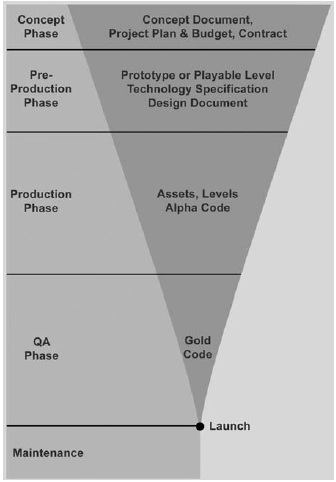
\includegraphics[scale=0.5]{./img/stages-game-development.jpg}
%  % matrixargseg.png: 296x162 pixel, 100dpi, 7.52x4.11 cm, bb=0 0 213 117~\cite{fullerton2008game}
%  %\caption{Estágio desenvolvimento de jogos ~\cite{fullerton2008game}}
% \caption[Fases de um processo de desenvolvimento de jogos dirigido a planos \copyright]{Fases de um processo de desenvolvimento de jogos dirigido a planos \copyright ~\cite{fullerton2008game}}
% %  \caption{Estágio desenvolvimento de jogos}
%  \label{fig:processoful}
% \end{figure}
% 
% Para Fullerton~\cite{fullerton2008game} no início do projeto as possibilidades criativas são grandes e por esse motivo durante essa fase ocorrem suscetíveis mudanças, porém ao longo do projeto devido a convergência de ideias e o progresso do desenvolvimento do jogo existe uma redução natural dessas modificações resultando no produto final~\cite{fullerton2008game} (Figura ~\ref{fig:processoful}).
% 
%  %For many games developed using agile, there is still a need to separate some of the development activities ~\cite{keith2010agile}. 
% \begin{figure}[!htbp]
%  \centering
%  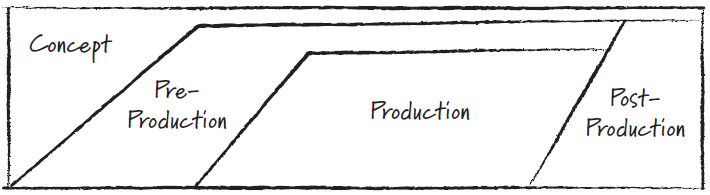
\includegraphics[scale=0.5]{./img/stages-game-development-agil.png}
%  % matrixargseg.png: 296x162 pixel, 100dpi, 7.52x4.11 cm, bb=0 0 213 117
%  %\caption{Estágio desenvolvimento de jogos ~\cite{fullerton2008game}}
% \caption[Fases de um processo de desenvolvimento ágil\copyright] {Fases de um processo de desenvolvimento ágil\copyright ~\cite{keith2010agile}}
% %  \caption{Estágio desenvolvimento de jogos}
%  \label{fig:processokeit}
% \end{figure}
% 
% 
% %inserir figura stages-game-development.png
% 
% %\subsubsection{Conceito}
% %Os requisitos para a concepção dos jogos sérios, o estímulo das funções cognitivas, a motivação e a aquisição de conhecimento são elementos fundamentais que precisam estar presentes ~\cite{machado_serious_2011}.
% 
% %Segundo Machado ~\cite{machado_serious_2011} os jogos sérios necessitam de uma colaboração estreita do especialistas da área de domínio em que o jogo está inserido. Essa colaboração irá permitir que as demais equipes responsáveis pelo desenvolvimento do jogo possam delinear o escopo do jogo e ainda assim inserir o conteúdo específico pertencente ao seu propósito ~\cite{ahn2008}.
% No desenvolvimento de um jogo tradicional, o principal objetivo da fase de conceito é conseguir o consenso entre todos os envolvidos com o primeiro marco de desenvolvimento. Infelizmente, o desenvolvimento de um jogo é uma atividade que possui muitos riscos devido sua complexidade, equipes de desenvolvimento mais experientes são mais indicadas para esses projetos~\cite{fullerton2008game}. No entanto, o desenvolvimento de um jogo com o objetivo de monitoramento de saíde possui um propósito específico logo na fase de conceito é necessário o apoio de profissionais especializados na área em que se pretende atuar. Incorporar esse profissional na equipe de desenvolvimento é necessário por permitir identificar quais serão os instrumentos e movimentos utilizados para a captura dos dados e como a coletado deve ser realizada para permitir uma melhor classificação dos dados.
% 
% Para o sucesso da abordagem deve-se pensar no público alvo e na equipe de desenvolvimento para mitigar os riscos do desenvolvimento de um jogo~\cite{fullerton2008game}. É durante a fase de conceito, em que serão testadas as tecnologias a serem utilizadas durante o desenvolvimento.
% 
% Abordagens tradicionais da engenharia de software sugerem que na fase inicial, sejam desenvolvidos protótipos de software com o objetivo de testar a tecnologia e verificar a viabilidade do projeto.
% 
% %pelo que estou lendo a fase de conceito, é para a escolha da equipe, demonstrar as capacidades técnicas e escolha da plataforma em que será desenvolvida e a habilidade do grupo naquela plataforma
% 
% %para o desenvolvimento do jogo seria interessante na fase de concepção, avaliarmos que enfermidades iríamos monitorar e avaliar as possíveis técnicas de monitoramento e testar as tecnologias que permitisse esse monitoramento.
% 
% 
% %\subsubsection{Pré-Produção}
% Na fase de pré-produção, um time pequeno faz um estudo de viabilidade da ideia. Esse time irá criar normalmente um ambiente jogável, focando nas possibilidades e riscos da tecnologia~\cite{fullerton2008game}.  A entrega de uma versão inicial que demonstre: a relevância da ideia, capacidade técnica da equipe de desenvolvimento  e os elementos de jogabilidade e diversão do jogo  são fatores cruciais para o prosseguimento nas demais etapas do processo de desenvolvimento~\cite{fullerton2008game}.
% Por se tratar de um jogo para o monitoramento, os desenvolvedores devem avaliar a capacidade de aquisição e classificação dos dados de saúde. O jogo deve ser divertido mas com o objetivo principal de adquirir dados de saúde.
% Como o estágio de pré-produção não é uma fase de construção de \textit{software}, é importante refinar o \textit{game design} do jogo, para que a documentação não fique desatualizada reduzindo os riscos potenciais do produto final~\cite{fullerton2008game}.
% 
% %\subsubsection{Produção}
% A fase de produção é a mais demorada e onerosa do desenvolvimento, o  seu objetivo é desenvolver o que foi pré-estabelecido no \textit{game design}. Nesse processo, o refinamento e melhoria do \textit{game design} é inevitável, pois os desenvolvedores passam mais tempo pensando nas soluções e consequentemente as reflete no \textit{game design}~\cite{fullerton2008game}. Nesse estágio os desenvolvedores escrevem o código criando as funcionalidades do jogo, os \textit{art designers} criam as artes e animação e os engenheiros de som criam as músicas e os efeitos sonoros, os responsáveis pelo enredo criam os diálogos e todo o contexto do jogo. A produção do jogo deve trabalhar de forma comunicativa e colaborativa para quer todos percebam o progresso do desenvolvimento do jogo~\cite{fullerton2008game}.
% 
% %\subsubsection{Pós-Produção}
% Na fase final do processo de desenvolvimento de jogos tradicionais a pós-produção é responsável por fazer o refinamento e últimos testes. Essa fase deve garantir que o jogo seja entregue com qualidade e sem erros de execução e que venha a impactar na jogabilidade. Nesse momento o jogo será testado nas diferentes plataformas para aprovar e e por fim disponibilizá-lo~\cite{keith2010agile}.

\section{Doença de Parkinson}\label{section:doenca_parkinson}
O termo Parkinsonismo é genérico e designa uma série de doenças com causas diferentes, que têm em comum a presença de sinais frequentemente encontrados no~\ac{dp}. Esta doença é uma das muitas formas de parkinsonismo, correspondendo a cerca de 75$\%$ dos casos. Os sinais associados ao~\ac{dp}~\cite{protpar010} são causados pela degeneração dos neurônios dopaminérgicos presentes na substância negra. O~\ac{dp} é mais comum em idosos, porém, existem casos precoces de início da doença em indivíduos antes dos 40 anos ou até mesmo abaixo dos 21~\cite{menezes2003}. A incidência da doença é estimada de 100 a 200 casos por 100.000 habitantes e com o avanço da idade populacional o contingente de pessoas diagnosticadas com ~\ac{dp} tende a aumentar.

O~\ac{dp} é uma doença progressiva e incapacitante e, após os 10 anos de tratamento: o custo operacional, impacto social e financeiro aumentam vertiginosamente. Estima-se, que o custo anual mundial com medicamentos antiparkinsonianos esteja em torno de 11 bilhões de dólares, tornando-se de de 3 a 4 vezes mais caro nas fases avançadas da doença~\cite{protpar010}. Outro fator crucial para a escolha do~\ac{dp} como objeto de estudo, é a variação dos sinais parkinsonianos ao longo do dia em virtude da resposta ao tratamento medicamentoso. Portanto, a abordagem de monitorar os sinais, em diferentes momentos do dia, permite um melhor gerenciamento da doença e, como consequência uma melhora na qualidade de vida dessa população.


Atualmente, o levodopa é o tratamento medicamentoso mais utilizado para o tratamento de redução dos sinais do~\ac{dp}. Porém, sua efetividade é reduzida ao longo do tempo, o que requer um aumento progressivo das dosagens ou uso de outros tratamentos associados. Isto acarreta num gerenciamento complexo entre drogas e seus respectivos efeitos colaterais. Portanto, ao buscar prolongar a qualidade de vida dos pacientes com o uso deste tratamento, é recomendável um gerenciamento medicamentoso com uma dosagem mínima~\cite{national2006parkinson} para: reduzir os sinais motores e prolongar a qualidade de vida do paciente. Como o gerenciamento medicamentoso é de responsabilidade do neurologista, este o faz de acordo com as visitas clínicas do paciente, quando estes ou seus cuidadores fazem relatos sobre o progresso do tratamento. Contudo, esta avaliação clínica é realizada de forma esporádica e de forma subjetiva~\cite{protpar010,quantitativeparkinson2011}. Desta maneira, é necessário uma quantificação destes sinais 
para um tratamento mais adequado e preciso. 

Com o surgimento do tratamento para o \ac{dp} é possível manter uma mobilidade funcional durante anos além de aumentar a expectativa de vida dos pacientes tratados~\cite{rodrigues2006}. Os fármacos do grupo dos antiparkinsonianos como a levodopa permitem restaurar a atividade dopaminérgica que se encontra reduzida, desta maneira as drogas aliviam os sinais característicos da doença. Entretanto, devido aos efeitos colaterais frequentes induzidos pelos fármacos, é preciso iniciar o tratamento com esses medicamentos somente quando os sinais estiverem prejudicando o desempenho profissional ou nas atividades diárias do paciente~\cite{rodrigues2006}. A natureza progressiva do~\ac{dp} e suas manifestações clínicas (motoras e não motoras), estão associadas a efeitos colaterais precoces e tardios da intervenção terapêutica, o que torna o tratamento da doença bastante complexo~\cite{protpar010}. Estima-se que a taxa de morte dos neurônios dopaminérgicos da substância negra situa-se 
ao redor de 10$\%$ ao ano~\cite{national2006parkinson}. Consequentemente, com o passar do tempo, a sintomatologia parkinsoniana tende a evoluir o que aumenta a necessidade de uma maior dosagem medicamentosa, pois a resposta aos medicamentos decresce com o progresso da doença~\cite{protpar010}.

%Na evolução da doença e pela tomada do medicamento pode existir alternância entre momentos em que a medicação surte efeito e momentos em que se torna ineficaz são os chamados estados \textit{on} e \textit{off}. Alternar entre os estados \textit{on} (''normal'') e \textit{off} (``com os sinais parkisonianos'') podem depender do horário da ingestão do medicamento que tornará previsível a mudança para o estado \textit{on}. Contudo, alguns pacientes podem ter mudanças abruptas para o estado \textit{off}, sem qualquer correlação com o tempo em que a medicação foi ingerida. Essa irregularidade indetermina o momento em que o paciente entrará no estado \textit{on} ou \textit{off} e esse efeito causa impacto direto nas avaliações objetivas do profissional~\cite{patel_monitoring_2009,kostek12}.

%%Outro efeito colateral no uso do medicamento bastante conhecido é o surgimento da discinesia (movimentos involuntários de contorção) em 80$\%$ dos pacientes que recebem a levodopa como tratamento prolongado. Esse sintoma pode ser aliviado com a diminuição da dose, por outro lado, os sinais da doença tendem a retornar. Com o surgimento de discinesia intensa é necessário otimizar o gerenciamento do tratamento medicamentoso, levando a adicionar novos medicamentos para reduzir os sinais incapacitantes a longo prazo ~\cite{rodrigues2006}. 
 
\subsection{Diagnóstico}
Os mais característicos do ~\ac{dp} e que são frequentemente usados para diagnosticar a doença são~\cite{rowlandtratado}: tremor em repouso (que diminui durante movimentos voluntários); bradicinesia ou hipocinesia (lentidão e escassez de movimentos, além de dificuldade na marcha), rigidez muscular (aumento da resistência ao movimento passivo dos membros), perda de reflexos posturais, que leva à alteração da marcha e aumenta a ocorrência de queda~\cite{rodrigues2006,tolosa06}. 

A evolução da doença, a gravidade e a progressão dos sinais variam de um paciente para outro. Atualmente, não existe teste diagnóstico estabelecido para a doença e, os estudos comprovam dificuldade na diferenciação clínica entre o~\ac{dp} e outras formas de parkinsonismo. A maioria dos neurologistas concordam que o diagnóstico do~\ac{dp} requer a identificação de alguma combinação de sinais motores cardinais como :tremor de repouso, bradicinesia, rigidez tipo roda denteada e alterações posturais. No entanto, uma classificação clínica padrão ainda não foi obtida ~\cite{protpar010}. Além do mais, um diagnóstico auxiliar importante é a resposta dos pacientes aos medicamentos antiparkinsonianos tal como a levodopa~\cite{protpar010}. Os protocolos clínicos~\cite{protpar010,national2006parkinson} sugerem que o diagnóstico do~\ac{dp} está diretamente relacionado à resposta satisfatória ao levodopa. No entanto, uma resposta satisfatória à levodopa não confirma o diagnóstico do~\ac{dp}~\cite{rowlandtratado}, porque 
existem muitos casos de parkinsonismo sintomáticos e, muitas formas de síndromes de Parkinson, que em seus estágios iniciais, respondem bem ao levodopa. 

Atualmente, os critérios estabelecidos pelo Banco de Cérebros da Sociedade de Parkinson do Reino Unido, são os mais utilizados para diagnosticar a doença~\cite{protpar010} (Apêndice \ref{apendice:diagnostico_parkinson}). 

%Como pouemos perceber ao longo desta seção, os estudos demonstram as dificuldades na diferenciação clínica entre o ~\ac{dp} e outros tipos de parkinsonismos. No entanto, através da revisão de diagnósticos patológicos e clínicos, um grupo de neurologistas especializados em distúrbios de movimento do \textit{National Hospital for Neurology and Neurosurgery} de Londres, conseguiu um valor preditivo de diagnóstico da doença em 98,6$\%$. 


\subsection{Principais Sinais do Parkinson}
Nesta seção serão descritos sintomas motores mais frequentes do~\ac{dp}~\cite{protpar010} e que foram objetos deste estudo. %\subsubsection{Prevenção de Flutuações Motoras e Discinesias}
%Um dos benefícios teóricos dos agonistas dopaminérgicos sobre a dopamina é uma meia-vida longa, resultando em menor estimulação pulsátil dos receptores de dopamina, o que poderia reduzir o risco do desenvolvimento de flutuações motoras e discinesias ~\cite{protpar010}.
%
%Os pacientes tratados com levodopa apresentam maior número de flutuações motoras e discinesias do que os tratados com pramipexol e cabergolina ~\cite{rasc2000,rinne98}. No entanto, estas diferenças entre agonistas e levodopa parecem desaparecer a longo prazo, pois estudos com mais de uma década de seguimento sugerem que os pacientes acabam tendo a mesma frequência de complicações motoras independentemente do tratamento que receberam nos primeiros anos da doença ~\cite{haus07,katzen08}. Com base nestes dados, tem sido recomendado que indivíduos mais jovens iniciem o tratamento sintomático com os agonistas da dopamina, por apresentarem maior risco das complicações motoras com levodopa ~\cite{silv98,acaneuro02,koll02}. Porém, se os sinais motores não forem bem controlados com doses adequadas de agonistas dopaminérgicos, levodopa deve ser logo adicionada a eles.

\subsubsection{Tremor}\label{sec:tremor}
O tremor é o sintoma mais frequente e mais perceptível~\cite{limongi2002} do~\ac{dp}, embora não seja o mais incapacitante. No entanto, para a maioria dos pacientes, este sinal é o principal motivo que os leva à procurar ajuda médica. Apresentando-se de forma característica: rítmico, relativamente lento quando comparado a outros tipos de tremor (4 a 7 ciclos por segundo), onde sua maior frequência é quando o membro está em repouso, sendo denominado de tremor de repouso. No início da enfermidade, o tremor ocorre em um lado (tremor assimétrico), e assim permanece por diferentes período de tempo. Situações de estresse emocional ou a sensação de ser observado, aumentam, visivelmente, a intensidade do tremor~\cite{jankovic2008}. 

Por ser um sinal relacionado ao repouso do membro, os usuários cessavam o sinal assim que eram confrontados com um jogo eletrônico desenvolvido para quantificação do tremor. Por esse motivo, não foi possível desenvolver um jogo que quantificasse este sinal.


\subsubsection{Bradicinesia}\label{section:analise_bradicinesia}
Enquanto que o sintoma de tremor é mais visível do~\ac{dp}, a bradicinesia é o sintoma mais incapacitante da doença. A bradicinesia consiste numa lentidão do movimento voluntário e num comprometimento de todos os movimentos associados a ele. A acinesia é uma progressão da bradicinesia e implica na ausência completa do movimento voluntário, sem a perda da força muscular~\cite{do2007parkinson}.

A bradicinesia pode estar presente nos sinais iniciais do~\ac{dp}, em diferentes partes do corpo: olhos com a redução do movimento de piscar, face com a redução das expressões faciais, voz robótica devido a redução da velocidade dos músculos das cordas vocais e membros(superiores e inferiores)~\cite{do2007parkinson}. Normalmente, nos estágios iniciais da doença, a bradicinesia é acompanhada de: rigidez dos músculos, assimetria dos movimentos entre os membros e dificuldade nos movimentos (levantar de uma cadeira, virar na cama ou andar). Os sinais bradicinéticos são avaliados por intermédio da parte motora da tabela de avaliação UPDRS~\cite{updrs87}, através de exercícios como tocar as pontas dos dedos, pronação e supinação do antebraço. 

\subsection{Escalas e os Estágios da Doença}\label{section:escalas_avaliacao}
A partir dos tratamentos para a~\ac{dp}, foram criadas escalas de avaliação do progresso da doença~\cite{updrs87,Hoehn_Yahr_2001}. Essas escalas permitem avaliar: a condição clínica geral, incapacidades, funções motoras, mentais e até mesmo a qualidade de vida dos pacientes. Esses instrumentos são importantes tanto no nível clínico quanto no científico, pois permitem monitorar a progressão da doença e a eficácia do tratamento medicamentoso~\cite{updrs87,goul05}.  Por conseguinte, foi criada em 1987 a Escala Unificada de Avaliação da  Doença de Parkinson (\textit{Unified Parkinson’s Disease Rating Scale – UPDRS})~\cite{updrs87} que é amplamente utilizada para monitorar o progresso da doença e a eficácia do tratamento. Segundo Goulart~\cite{goul05}, as escalas de estágios de incapacidade representadas por: \textit{Hoehn/Yahr}~\cite{Hoehn_Yahr_2001} e a \textit{UPDRS}~\cite{updrs87}, são consideradas as de maior confiabilidade, podendo ser usadas por fisioterapeutas para melhor avaliação do estado clínico-
funcional do  paciente.% 
% Atualmente a evolução da \ac{dp} é avaliada através de escalas, que permitem avaliar a eficácia do tratamentos e sua aplicabilidade nas práticas fisioterápicas. Segundo um trabalho de Goulart ~\cite{goul05} as escalas de estágios de incapacidade representadas por Hoehn/Yahr ~\cite{Hoehn_Yahr_2001} e a UPDRS ~\cite{updrs87} são consideradas as de maior confiabilidade, podendo ser usadas por fisioterapeutas para melhor avaliação do estado clínico-funcional do  paciente.

Segundo a \textit{UPDRS}, a evolução do~\ac{dp} é classificada nas seguintes fases ~\cite{updrs87}:
  \begin{itemize}
    \item \textbf{ESTÁGIO 0:} Nenhum sinal da doença;
    \item \textbf{ESTÁGIO 1:} Doença unilateral;
    \item \textbf{ESTÁGIO 1,5:} Envolvimento unilateral e axial;
    \item \textbf{ESTÁGIO 2:} Doença bilateral sem déficit de equilíbrio;
    \item \textbf{ESTÁGIO 2,5:} Doença bilateral leve, com recuperação no “teste do empurrão”;
    \item \textbf{ESTÁGIO 3:} Doença bilateral leve a moderada; alguma instabilidade postural; capacidade para viver independente;
    \item \textbf{ESTÁGIO 4:} Incapacidade grave, ainda capaz de caminhar ou permanecer de pé sem ajuda;
    \item \textbf{ESTÁGIO 5:} Confinado à cama ou à cadeira de rodas.
  \end{itemize}

A \textit{UPDRS} é composta por 42 itens, divididos em quatro partes: atividade mental; comportamento e humor; atividades de vida diária; exploração motora e complicações da terapia medicamentosa. Estes itens, são avaliados por auto-relato ou observação clínica. Desta maneira, subjetiva, é realizada a classificação do estágio da doença no paciente. Contudo, justamente por ser baseada em auto-relato e observação clínica, a qual é realizada eventualmente com a presença de um profissional, pesquisadores questionam a efetividade da análise do estágio da doença e, propõem alternativas para avaliação dos itens motores de forma quantitativa, através de sensores, os quais permitem quantificar os sinais motores do paciente~\cite{kostek12,synnott_wiipd_2012,patel_monitoring_2009}.

%Alguns sinais parkisonianos são consequências do longo período do uso da medicação seja ela levodopa ou dopaminérgicos~\cite{protpar010}. No início do tratamento, o levodopa irá melhorar consideravelmente a qualidade de vida do paciente e poderá permanecer nesse estado por anos. Mas com o passar dos anos a efetividade do levodopa diminuirá e o paciente irá alternar entre os estados \textit{on} e \textit{off}. Por esse motivo, a detecção das alterações dos estágios da doença dentro de curtos períodos é complicada, em particular porque os testes a partir das escalas são aplicados de forma objetiva por um profissional, que avalia  evolução do quadro periodicamente de três a seis meses. Isso se torna um obstáculo tanto para o paciente quanto a disponibilidade do profissional, deve ser mencionado também que a precisão da avaliação dependerá das capacidades motoras e do tempo em que o medicamento foi ingerido.
% (``com os sinais parkisonianos''). As mudanças dos estados \textit{on} para \textit{off} dependerá do agendamento da ingestão do medicamento que tornará previsível a mudança para o estado \textit{on}. Contudo, alguns pacientes, podem ter mudanças abruptas para o estado \textit{off}, sem qualquer correlação com o tempo em que a medicação foi ingerida, isso é chamado do fenômeno \textit{on-off} e mudanças do estado \textit{on} ou \textit{off} podem ocorrer [~\cite{patel_monitoring_2009}. Essa irregularidade de não conseguir determinar o momento em que o paciente entrará no estado \textit{on} ou \textit{off} impacta diretamente nas avaliações objetivas do profissional que irá avaliar os estágios da doença fazendo uma avaliação errada ~\cite{patel_monitoring_2009}.

A identificação dos sinais do~\ac{dp} durante a rotina diária, permite um diagnóstico mais precoce da doença e, consequentemente, obter os benefícios de um tratamento mais duradouro. Além disso, o monitoramento dos efeitos da medicação junto ao paciente, permite um melhor gerenciamento medicamentoso e, assim, reduz os efeitos colaterais do tratamento e prolonga sua qualidade de vida~\cite{rowlandtratado}.


\section{Cinemetria}
A \textbf{Cinemetria} consiste em um conjunto de métodos para medição dos parâmetros cinemáticos do movimento como: posição, orientação, velocidade e aceleração~\cite{biomecanica99}. Os instrumentos básicos das medidas cinemáticas podem ser adquiridos por: câmeras de vídeo; durante a análise das imagens e dos movimentos; por meio de software específico, os quais calculam as variáveis cinemáticas de interesse. Atualmente, com o uso de câmeras infravermelho, é possível reconhecer o movimento humano e calcular as grandezas cinemáticas das características do movimento com precisão e robustez~\cite{gabel2012}.

A cinemetria relaciona técnicas e métodos para o processamento de grandezas cinemáticas, entre elas, destacamos as técnicas de medição direta~\cite{biomecanica99}, utilizadas para: 
\begin{enumerate}
	\item medidas de tempo;
	\item medidas de ângulos;
	\item medidas de amplitude;
	\item medidas de velocidade angular.
\end{enumerate}

% \subsection{Movimento Cinético}
% Movimento Cinético é o estudo das forças e momentos que resultam no movimento do corpo e seus segmentos, incluindo a mensuração da \ac{fvrs} e análise cinética. A Medição Cinética é realizada das forças presentes entre o pé e o solo, a qual é medida por intermédio de sensores de força que permitem adquirir a pressão do pé em relação ao solo. Estudos indicam que por meio da análise do movimento cinético é possível avaliar o desempenho do corpo durante a execução das atividades diárias~\cite{gaitusingsensorsreview2012}.
% 
% Nos últimos anos com os sensores de movimento vestíveis, foi possível evoluir os estudos sobre a análise de marcha em ambientes que não fossem somente os laboratórios e clínicas, os quais possuíam placas de força e esteiras eletrônicas que permitem realizar o estudo~\cite{gaitusingsensorsreview2012}. Pode ser salientado também, que por meio destes dispositivos o monitoramento contínuo da marcha pode ser possível mensurar e quantificar os ciclos de movimento de cada usuário na sua rotina diária e consequentemente identificar sinais relativos a marcha.


%==========================
% Sensores
%==========================
%In gait analysis using wearable sensors, motion sensors are worn or attached to various parts of the patient’s body, such as the foot and waist. These sensors, which may be accelerometers, gyrosensors, force sensors, strain gauges, inclinometers, goniometers, and so on, can measure various characteristics of the human gait [20,21]. The movement signal recorded by these sensors can be used to perform the gait analysis ~\cite{gaitusingsensorsreview2012}.

%-------------------------------
%2.2.1. Accelerometer, Gyroscope, and Magnetoresistive Sensors
%-------------------------------
%An accelerometer is a type of inertial sensor that can measure acceleration along its sensitive axis. The common operation principle of accelerometers is based on a mechanical sensing element that comprises a proof mass attached to a mechanical suspension system, with respect to a reference frame.
%The mass proof can be forced to deflect by the inertial force because of acceleration or gravity according to Newton’s second Law (force = mass × acceleration). Based on this principle, the acceleration can be measured electrically using the physical changes in the displacement of the proof mass, with respect to the reference frame.
%Three common types of accelerometers are available, namely, piezoelectric, piezoresistive, and capacitive accelerometers [35]. Piezoresistive and capacitive accelerometers can provide dual acceleration components and have higher stability. Thus, these types of accelerometers are suitable for measuring the motion status in the human gait [36]. By attaching these accelerometers to the feet or legs, the acceleration/velocity of the feet or legs in the gait can be determined to perform the gait analysis [37].
%~\cite{gaitusingsensorsreview2012}

%Force Sensors
----------------------------
%----------------------------------
% Attention here he talks about vertical ground reaction forces
%----------------------------------
%Slavelberg and Forner-Cordero reported on estimates of the three-dimensional (3D) ground reaction forces (GRFs) from the insole based on foot pressure data [28,29]. With the development of motion-sensing technology, an increasing number of wearable sensors will be developed for gait analysis in the future. Gait analysis using wearable sensors will thus be widely used in the clinical field.
%~\cite{gaitusingsensorsreview2012}

%Force sensors can be embedded into footwear to realize ambulatory measurements of GRF during the gait. This GRF is a 3D vector, with the actual direction depending on the nature of the interface between the foot and the ground. In the development of wearable force sensors, various implementations of the force transducer, including piezoelectrics [68,69], strain gauged [70,71] and capacitive transducerd [72–74], are feasible. In addition, Hessert et al. designed a type of wearable force sensor based on a photoelastic triaxial force transducer to measure GRF in gait analysis [75]. Force sensors based on the optical fiber matrix were developed to detect the shear and compressive force during human walking [76,77].
%~\cite{gaitusingsensorsreview2012}

%---------------------------
% Kinnect
%---------------------------
%We propose a low-cost, non-intrusive system that can accurately measure a wide range of gait parameters using the Kinect sensor and Software Development Kit (SDK). Kinect is an array of sensors, including a camera and a depth sensor. In addition to the raw depth image, Kinect extracts a 3D virtual skeleton of the body [17]. These capabilities, packed in an affordable and compact device, already led several researchers to propose its use for home monitoring and gait analysis [18], [19].
%We apply a supervised learning approach to automatically and accurately extract lower and upper body gait parameters, using the 3D virtual skeleton. This allows us to go beyond standard foot stride parameters. For example, we extract arm kinematics using the same sensor. We show that our method is accurate and robust to attributes such as sensor position. Moreover, our method can be extended to measure other properties such as leg kinematics.
%In this work we have presented a novel method for full body gait analysis using the Kinect sensor. Using the virtual skeleton as the input to a learned model, we demonstrated accurate and robust measurements of a rich set of gait features.In this work we have presented a novel method for ful body gait analysis using the Kinect sensor. Using the virtual skeleton as the input to a learned model, we demonstrated accurate and robust measurements of a rich set of gait features.
%~\cite{gabel2012}


%===========================
%Dificuldades
%==========================


%===========================
%4. Application of Gait Analysis Using Wearable Sensors
%===========================
%With the development of sensor technology and gait data analyzing techniques, gait analysis using wearable sensors has become a widespread and useful tool for both clinical practice and biomechanical research. Using small, low-power, and low cost wearable sensors, ambulatory gait analysis can be used conveniently in sports, rehabilitation, and clinical diagnostics, as summarized in the following. %~\cite{gaitusingsensorsreview2012}

% 4.3. Clinical Diagnosis and Healthcare Monitoring
%In the clinical diagnosis of patients with Parkinson’s or knee osteoarthritis disease, the ambulatory estimation of lower extremity movement in the gait is usually necessary [172]. Based on the estimation results of the lower extremities, the disease and its severity can be determined, and clinicians can establish a proper treatment scheme for the patients. In healthcare monitoring, gait analysis based on wearable sensors can also be applied in various occasions, such as in the detection of gait abnormalities, the assessment of recovery, fall risk estimation, and so on. In the healthcare environment, gait information is used to detect walking behavior abnormalities that may indicate the onset of adverse health problems or the progression of neurodegenerative diseases [173]. The presence of gait abnormalities in elderly persons is often a significant predictor of the risk of the development of dementia, especially non-Alzheimer’s dementia [174].
%~\cite{gaitusingsensorsreview2012}

%Passos para análise

\subsection{Movimento Angular}
O movimento angular ocorre quando todas as partes do corpo se movem pelo mesmo ângulo mas não realizam o mesmo deslocamento linear. A subdivisão da cinemática que trata do movimento angular é chamada de cinemática angular, que permite examinar o movimento angular a partir de segmentos de um movimento, divididos em partes identificáveis que aumentam a compreensão do movimento humano~\cite{hamill1999bases}. 

Quase todos os movimentos humanos envolvem as rotações de segmentos do corpo, os segmentos giram sobre os centros articulares que formam os eixos de rotação para esses segmentos~\cite{hamill1999bases}. No movimento angular, a unidade de medida utilizada é o grau (º) e a unidade de tempo é o segundo (s). Logo, as velocidades angulares calculadas são mensuradas em °/s.

A anatomia funcional consiste no estudo dos componentes do corpo, necessários para desempenhar um movimento ou função humana como, por exemplo, a abdução ou adução do braço (Figura \ref{fig:movabducaoaducao}).

\begin{figure}
 \centering
 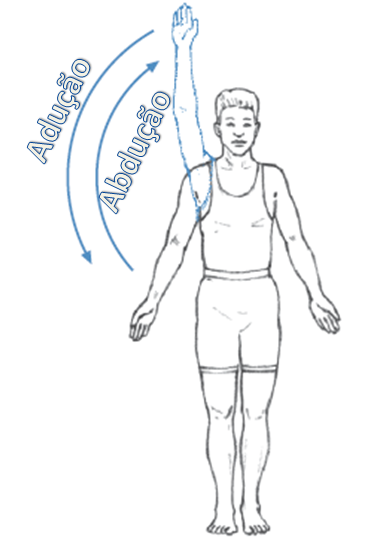
\includegraphics[scale=0.5]{./img/abducao.png}
 % matrixargseg.png: 296x162 pixel, 100dpi, 7.52x4.11 cm, bb=0 0 213 117
 %\caption{Estágio desenvolvimento de jogos ~\cite{fullerton2008game}}
\caption[Movimentos de Abdução e Adução do Braço]{\copyright Movimentos de Abdução e Adução do Braço~\cite{mcginnis2013biomechanics}}
%  \caption{Estágio desenvolvimento de jogos}
 \label{fig:movabducaoaducao}
\end{figure}

Na análise biomecânica do movimento humano, são calculados dois tipos de ângulos:
	\begin{itemize}
		\item Ângulo Relativo: este ângulo é formado entre os eixos longitudinais de segmentos corporais adjacentes~\cite{hamill1999bases}. Logo, os ângulos relativos, não descrevem a posição de segmentos ou os lados do ângulo no espaço. Se um indivíduo tem um ângulo relativo de 90º no cotovelo e esse ângulo é mantido, o braço pode ficar em qualquer posição. A interpretação dada a cada segmento irá determinar o tipo de movimento realizado. 
		\item Ângulo Absoluto: este ângulo identifica a orientação angular de um segmento corporal em relação a uma linha fixa de referência~\cite{hamill1999bases}. Dessa forma, os ângulos absolutos devem ser medidos na mesma direção a partir de uma única referência, seja ela horizontal ou vertical.
	\end{itemize}


%A interpretação correta de flexionar o braço pode ser levantar todo o braço, já que braço refere-se ao úmero, não ao rádio e à ulna. Uma revisão dos nomes dos segmentos é indispensável no preparo para o uso mais extensivo deles no estudo da biomecânica ~\cite{hamill1999bases}.

\section{Máquinas de Vetor de Suporte (SVM)}\label{sec:svm_linear}
A teoria da aprendizagem estatística fornece um conjunto de técnicas para a análise de dados, a qual permite a aquisição de conhecimento~\cite{vapnik95}. As máquinas ~\ac{svm}, fazem uso de um conjunto de métodos de aprendizagem supervisionada para classificação de dados. Ou seja,~\ac{svm} é uma ferramenta de predição de classificação, que usa a teoria da aprendizagem de máquina e busca maximizar a acurácia. Normalmente, a~\ac{svm} é aplicada para classificação binária, ou seja, permite classificar os dados em duas classes. No entanto, essa técnica, também tem sido aplicada em dados com mais de duas classes~\cite{multisvm2011}.

Um classificador ~\ac{svm} foi inicialmente desenvolvido para problemas de aprendizagem linearmente separáveis e, utiliza vetores de separação, através de uma técnica de hiperplano de separação ótima ~\cite{vapnik95}. O hiperplano tenta separar as diferentes classes, maximizando a margem entre os pontos extremos de cada classe~\cite{valt2010}. O melhor hiperplano de uma~\ac{svm} é aquele que possui a maior margem entre as duas classes como pode ser visto na Figura ~\ref{fig:hiperplano}.  

\begin{figure}
 \centering
 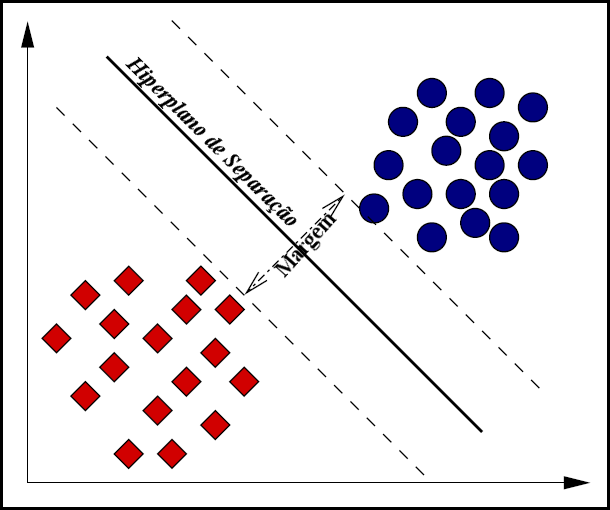
\includegraphics[scale=0.4]{./img/svmhyperplane.png}
 % matrixargseg.png: 296x162 pixel, 100dpi, 7.52x4.11 cm, bb=0 0 213 117
 %\caption{Estágio desenvolvimento de jogos ~\cite{fullerton2008game}}
\caption{Hiperplano de Separação Linear Para Duas Classes}
%  \caption{Estágio desenvolvimento de jogos}
 \label{fig:hiperplano}
\end{figure}


Para entender o funcionamento da ~\ac{svm} é necessário conhecer a notação:
\begin{math}
R^{n}
\end{math}
é um número real n-dimensional no espaço de vetores. Onde os pontos \textbf{u}, \textbf{v}, \textbf{w} e \textbf{x} serão utilizados para denotar pontos em 
\begin{math}
R^{n}
\end{math}.
Estes pontos são chamados de vetores ou padrões na literatura de Aprendizagem de Máquina.

Cada ponto possui $x_{i}$ e um rótulo $y_{i}$ que denota a qual classe $x_{i}$ pertence. Logo, se $y_{i} = + 1$ e $x_{i}$ pertencer a classe 1 e $y_{i} = - 1$ caso o $x_{i}$ pertencer a classe 2. A classificação binária como o nome sugere, significa classificar os dados em duas classes. Para tanto, primeiramente os dados do grupo de treinamento são usados para preencher os espaços com pontos. E depois um segundo grupo de teste é aplicado para verificar a hipótese de qual classe aquele ponto pertence. Formalmente, dado um conjunto de pontos $x_{i}$ qual será os valores $y_{i}$ correspondentes. Dado que o classificador possui os padrões adquiridos do grupo de treinamento além dos rótulos associados a sua classe. A~\ac{svm} irá usar o hiperplano de separação para tentar dividir os dados de treinamento em duas classes. Desta maneira, o resultado da classificação dos dados de teste dependerá da localização da projeção desses dados.

Formalmente, classificadores que separam os dados por meio de um hiperplano utilizam um discriminante linear~\cite{valt2010} de Equação~\ref{eq:hiperplano}. Um hiperplano é considerado de Margem Máxima (ou de Separação Ótima) quando separa um conjunto de vetores sem erro e a distância entre os vetores (das classes opostas) mais próximas ao hiperplano, é máxima por intermédio de uma função discriminante. Uma função é discriminante quando consegue discriminar os valores em diferentes padrões. 

O produto escalar $ w.x $ entre os vetores $ w $ e $ x $, $ w $ é o vetor normal ao hiperplano descrito, e o vetor \textbf{w} é denominado de peso e a constante parâmetro \textbf{b} é chamada de \textit{bias} ou desvio.
\linebreak
\begin{equation}
f(x)=w^Tx+b=0
\label{eq:hiperplano}
\end{equation}

Se \textbf{u} e \textbf{v} são dois padrões e \textit{f(x)} é a função discriminante, então os valores de \textit{f(\textbf{u})} e \textit{f(\textbf{v})} irá auxiliar em determinar se os valores de \textbf{u} e \textbf{v} pertencem a classe, logo, a regra para a predição da classe está no Código~\ref{codepredicaoclasse}. 

\begin{lstlisting}[frame=single, caption=Código de Predição da Classes, label=codepredicaoclasse]  % Start your code-block

classificacao = 0;
if (w^t.x + b > = 0)
	classificacao = 1
else
	classificacao = -1;
endif
\end{lstlisting}
A partir desse método de separação de dados lineares, é que a~\ac{svm} foi aplicada para classificar indivíduos diagnosticados com ~\ac{dp} ante indivíduos sem o diagnóstico estabelecido. Na Seção~\ref{sec:processador_bio}, será explicado como são extraídos os pontos, usando os vetores de características para obtenção da classificação exposta na Seção~\ref{sec:resultado_svm}.

